
\mode<presentation>
{
  \usetheme{CambridgeUS}
  \usecolortheme{whale}
  \usecolortheme{lily}

  \setbeamercovered{transparent}
  \usefonttheme[onlymath]{serif}
}

\title[\StabilityandRouthHurwitzShortName] 
{\course: \StabilityandRouthHurwitzName\license}

\subtitle
{Lecture \StabilityandRouthHurwitzNumber}



\begin{document}

\begin{frame}
  \titlepage
\end{frame}

\mode<article>{
\maketitle
\tableofcontents
}


\section{Pre-requisite Material}

This lecture assumes that the reader is familiar with the following material:
\begin{itemize}
\item Lecture \ImpedanceNumber:~\ImpedanceName
\end{itemize}



\section{Definition of Stability}
\begin{definition}
A system is {\em Bounded Input Bounded Output} (BIBO) {\em stable} if every bounded input results in a bounded output
\end{definition}

\begin{definition}
A rational transfer function $G(s)$ is {\em proper} if the number of poles is greater than or equal to the number of zeros 
\end{definition}

\begin{fact}
An LTI system with transfer function $G(s)$ is BIBO stable if and only if $G(s)$ is proper and all poles $p_{i}$ satisfy $\mbox{Re}\{p_{i}\}<0$.
\end{fact}

\begin{frame}{BIBO Stability Examples}
\begin{center}
\begin{tikzpicture}
\draw (0,1.75) node {BIBO stable};
\draw (0,0) node {
\begin{tikzpicture}[scale=.4]
\draw[->] (-6,0) -- (2,0) node[below=2pt] {Re$(s)$};
\draw[->] (0,-3) -- (0,3) node[left=2pt] {Im$(s)$};
\draw (-4,0) node {\Large\sf x};
\draw (-1,1) node {\Large\sf x};
\draw (-1,-1) node {\Large\sf x};
\end{tikzpicture}};

\draw (5,1.75) node {not BIBO stable};
\draw (5,0) node {
\begin{tikzpicture}[scale=.4]
\draw[->] (-6,0) -- (2,0) node[below=2pt] {Re$(s)$};
\draw[->] (0,-3) -- (0,3) node[left=2pt] {Im$(s)$};
\draw (1,0) node {\Large\sf x};
\draw (-1,1) node {\Large\sf x};
\draw (-1,-1) node {\Large\sf x};
\end{tikzpicture}};

\draw (2.5,-1.75) node {not BIBO stable};
\draw (2.5,-3.5) node {
\begin{tikzpicture}[scale=.4]
\draw[->] (-6,0) -- (2,0) node[below=2pt] {Re$(s)$};
\draw[->] (0,-3) -- (0,3) node[left=2pt] {Im$(s)$};
\draw (-4,0) node {\Large\sf x};
\draw (0,1) node {\Large\sf x};
\draw (0,-1) node {\Large\sf x};
\end{tikzpicture}};



\end{tikzpicture}
\end{center}
\end{frame}

\section{Test of Stability}

Given a proper rational transfer function
\[
G(s)=\frac{N(s)}{D(s)}
\]
the system represented by $G(s)$ is BIBO stable if all the roots of $D(s)$ are in the {\em open left half complex plane} (OLHP). These are the poles for which $\mbox{Re}\{s\}<0$.

\begin{enumerate}
\item[Step 1] Write $D(s)$ as
\[
D(s) = a_{0}s^{n} +a_{1}s^{n-1} + \cdots + a_{n-1}s +a_{n}.
\]
It is assumed that $a_{0}>0$ - if not, multiply $D(s)$ by $-1$ (does not change locations of roots).
\item[Step 2] Quick check - if any $a_{i}$ is negative, then there is at least one root with positive real part, and thus at least one root that is {\em not} in the OLHP.
\item[Step 3] If all coefficients are positive, there still may be roots outside of the OLHP. To determine for sure, form the Routh Array. The first two rows of the Routh array consist of the coefficients of $D(s)$. The remaining rows are each calculated using the two rows immediately prior.
\begin{frame}{Start of Routh Array}
\begin{center}
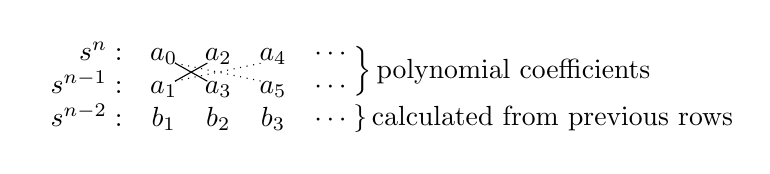
\begin{tikzpicture}
\draw (0,0) node {$\begin{array}{rcccc} s^{n}: & a_{0} & a_{2} & a_{4} & \cdots \\
s^{n-1}: & a_{1} & a_{3} & a_{5} & \cdots \\
s^{n-2}: & b_{1} & b_{2} & b_{3} & \cdots \end{array}$};
\draw (1.8,.2) node[right] {$\left.\rule{0pt}{12pt}\right\}\mbox{polynomial coefficients}$};
\draw (1.8,-.4) node[right] {$\left.\rule{0pt}{8pt}\right\}\mbox{calculated from previous rows}$}; 
\draw (-.3,.3) -- (.11,.07);
\draw (-.3,.07) -- (.11,.3);
\draw[dotted] (-.3,.3) -- (.8,.07);
\draw[dotted] (-.3,.07) -- (.8,.3);
\end{tikzpicture}
\[
b_{1} = \frac{a_{1}a_{2} - a_{0}a_{3}}{a_{1}} = \frac{-1}{a_{1}}\begin{vmatrix} a_{0} & a_{2} \\ a_{1} & a_{3}\end{vmatrix} \quad b_{2} = \frac{a_{1}a_{4} - a_{0}a_{5}}{a_{1}} \quad b_{3} = \frac{a_{1}a_{6} - a_{0}a_{7}}{a_{1}}
\]
\end{center}
\end{frame}
The remaining rows are calculated in the same way, until the number of rows is equal to the number of coefficients of $D(s)$. 
\begin{frame}{Routh Array Continued}
\begin{center}
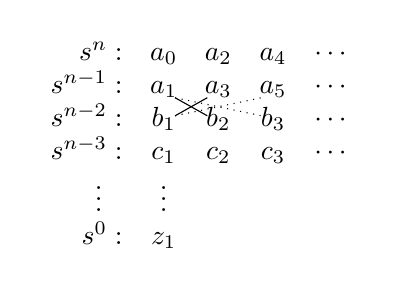
\begin{tikzpicture}
\draw (0,0) node {$\begin{array}{rcccc} s^{n}: & a_{0} & a_{2} & a_{4} & \cdots \\
s^{n-1}: & a_{1} & a_{3} & a_{5} & \cdots \\
s^{n-2}: & b_{1} & b_{2} & b_{3} & \cdots \\
s^{n-3}: & c_{1} & c_{2} & c_{3} & \cdots  \\
\vdots\hspace{.1in} & \vdots & & & \\
s^{0}: & z_{1} & & & \end{array}$};
\draw (-.3,.61) -- (.11,.38);
\draw (-.3,.38) -- (.11,.61);
\draw[dotted] (-.3,.61) -- (.8,.38);
\draw[dotted] (-.3,.38) -- (.8,.61);
\end{tikzpicture}
\end{center}
\[
c_{1} = \frac{b_{1}a_{3} - a_{1}b_{2}}{b_{1}} \quad c_{2} = \frac{b_{1}a_{5} - a_{1}b_{3}}{b_{1}} \quad \cdots
\]
\end{frame}

\item[Step 4] The number of roots with positive real part is equal to the number of sign changes in the first column. If any element of the first column is zero, then at least one pole has real part $\geq 0$.
\begin{frame}{Routh-Hurwitz Test: }{Last Step}
\begin{center}
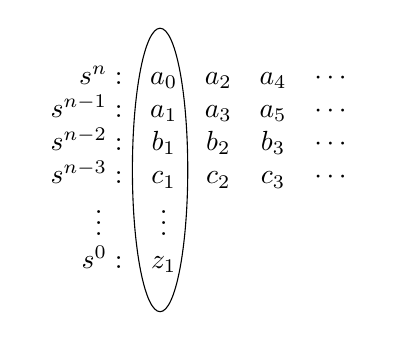
\begin{tikzpicture}
\draw (0,0) node {$\begin{array}{rcccc} s^{n}: & a_{0} & a_{2} & a_{4} & \cdots \\
s^{n-1}: & a_{1} & a_{3} & a_{5} & \cdots \\
s^{n-2}: & b_{1} & b_{2} & b_{3} & \cdots \\
s^{n-3}: & c_{1} & c_{2} & c_{3} & \cdots  \\
\vdots\hspace{.1in} & \vdots & & & \\
s^{0}: & z_{1} & & & \end{array}$};
\draw (-.49,0) circle [x radius=10pt, y radius=1.8cm]; 
\end{tikzpicture}
\end{center}
\end{frame}
\end{enumerate}

\begin{example} Determine the number of roots outside of the OLHP for the polynomial
\[
D(s) = 5s^{4} +4s^{3} +3s^{2} +2s+1
\]
\end{example}
\[
\begin{array}{rccc} s^{4}: & 5 & 3 & 1 \\
s^{3}: & 4 & 2 &   \\
s^{2}: & \frac{1}{2} & 1 &   \\
s^{1}: & -6  &  &    \\
s^{0}: & 1 & & 
\end{array}
\]
\[
b_{1} =\frac{12-10}{4} = \frac{1}{2} \quad b_{2} = \frac{4-0}{4} = 1 \quad c_{1} = \frac{1-4}{0.5} = -6 \quad d_{1} =\frac{-6 -0 }{-6} = 1 
\]
Two sign changes - 2 RHP roots.

\begin{example} Find the allowable range of the gain $K$ for a stable closed loop system for the following feedback system
\begin{frame}
\begin{center}
\input{figures/feedbackexample.tex}
\end{center}
\mode<article>{\textbf{Solution:} First, find the closed loop transfer function.}
\visible<2->{\begin{align*}
\frac{Y(s)}{R(s)} &= \frac{K\frac{s}{s^{4}+s^{3}+6s^{2}+1}}{1+K\frac{s}{s^{4}+s^{3}+6s^{2}+1}} \\
&=\frac{Ks}{s^{4}+s^{3}+6s^{2}+Ks+1}
\end{align*}}
\end{frame}
The denominator of the closed loop system depends on $K$. The Routh array for this denominator is
\begin{frame}
\[
\begin{array}{rccc} s^{4}: & 1 & 6 & 1 \\
s^{3}: & 1 & K &   \\
s^{2}: & 6-K & 1 &   \\
\visible<2->{s^{1}: & K-\frac{1}{6-K}  &  &    \\}
\visible<3->{s^{0}: & 1 & &} 
\end{array}
\]
\end{frame}
The requirements for stability are that the elements in the first column are all positive. This requires
\begin{align*}
6-K&>0\\
K-\frac{1}{6-K} &>0
\end{align*}
The second inequality can be simplified. Since we already require $6-K>0$, we can multiply both sides of the second inequality by this positive term without affecting the inequality
\begin{align*}
(6-K)K - (6-K)\frac{1}{6-K} & > 0(6-K)\\
K(6-K) - 1&>0\\
-K^{2} + 6K - 1&>0
\end{align*}
This is the equation for a downward facing parabola, as shown in the following figure
\begin{frame}
\mode<presentation>{\[
-K^{2} + 6K - 1>0
\]}
\begin{center}
\includegraphics[width=3in]{figures/exampleparabola}
\end{center}
\end{frame}
This parabola is positive between the roots, which are found using the quadratic formula
\[
K=3\pm\sqrt{8} = .172, 5.8
\]
The requirements for stability are thus
\[
.172 < K < 5.8 \quad \mbox{and} \quad K<6
\]
The overall requirement is the intersection of these two sets, which is
\[
.172 < K < 5.8
\]
\end{example}

\section{Lecture Highlights}
The primary takeaways from this article include
\begin{enumerate}
\setlength{\itemsep}{5pt}
\setlength{\parskip}{0pt}
\setlength{\parsep}{0pt}
\item Stability is one of the key topics in control systems. Make sure you understand both Definition 1 and Fact 3 of this lecture. 
\item The Routh Hurwitz test is a tool that can be used to test for stability of systems. It is most useful when either the system cannot be easily factored (to find the pole values and determine whether or not they are in the left half plane) or when finding an allowable range for a parameter that would result in a BIBO stable system. If numeric pole locations can be determined, it is not necessary to apply the Routh Hurwitz test.
\end{enumerate}


\section{Quiz Yourself}

\subsection{Questions}


\begin{enumerate}
\setlength{\itemsep}{5pt}
\setlength{\parskip}{0pt}
\setlength{\parsep}{0pt}
\item Determine if the following system is BIBO stable using the Routh-Hurwitz test
\[
G(s) = \frac{s-6}{s^{4}+3s^{3}+3s^{2}+3s+1}
\]
\item Determine if the following system is BIBO stable using the Routh-Hurwitz test
\[
G(s) = \frac{s^2+3s+6}{s^{4}+3s^{3}+3s^{2}+3s+4}
\]
\end{enumerate}


\subsection{Solutions}
\begin{enumerate}
\setlength{\itemsep}{5pt}
\setlength{\parskip}{0pt}
\setlength{\parsep}{0pt}
\item \rule{0pt}{12pt}\\
\begin{center}
\includegraphics[width=5in]{quizfigures/1soln}\\
\end{center}\pagebreak
\item \rule{0pt}{12pt}\\
\begin{center}
\includegraphics[width=5in]{quizfigures/2soln}\\
\end{center}

\end{enumerate}


\section{Resources}

\subsection{Books}


\begin{itemize}
\item Norman S. Nise, {\em Control Systems Engineering}, Wiley
\begin{itemize}
\item 7th edition: Sections 6.1-6.2
\end{itemize}
\item Richard C. Dorf and Robert H. Bishop, {\em Modern Control Systems}, Pearson
\begin{itemize}
\item 13th edition: Sections 6.1-6.2
\end{itemize}
\item Gene F. Franklin, J. David Powell and Abbas Emami-Naeini,  {\em Feedback Control of Dynamic Systems}, Pearson
\begin{itemize}
\item 6th and 7th edition: Section 3.6
\end{itemize}
\end{itemize}


\subsection{Web resources}

If you find any useful web resources, please contact your instructor.



\end{document}


